%\documentclass[a4paper,12pt]{article}
\documentclass[convert={density=300}]{standalone}
\pagestyle{empty}
\usepackage{pst-plot}
\usepackage{color}
\usepackage{tikz}
\usepackage{amsmath}
\usetikzlibrary{automata,positioning}
\definecolor{bael1}{RGB}{99,177,117}

\begin{document}
\newlength{\w}
\setlength{\w}{1cm}


% \begin{tikzpicture} 
%  \draw (0, 0) node[minimum height=1cm, minimum width=1cm, color=gray, draw](n1) {n} 
%        (1.5, 0) node[minimum height=1cm, minimum width=1cm, color=gray, draw](n2) {n${}^2$}
%        (3.5, 0) node[minimum height=1cm, minimum width=1cm, color=bael1, draw](n3) {extract\\ middle}; 

% \draw[->, gray] (n1)--(n2);
% \draw[->] (n2)--(n3);
% \draw[->] (n3.south) to[out=-90, in=-90] node{repeat} (n1.south);
% \end{tikzpicture}


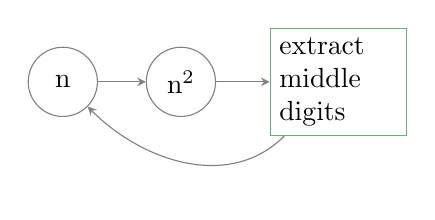
\begin{tikzpicture}[>=stealth, node distance=1.5cm, on grid, auto]
    \node[state] (n1) [draw=gray]              {n};
    \node[state] (n2) [right of=n1, draw=gray] {n${}^2$};
    \node        (n3) [right of=n2, draw=bael1, text width=1.5cm] at (2, 0) {extract middle digits};
\draw[->, gray] (n1)--(n2);
\draw[->, gray] (n2)--(n3);
\draw[->, gray] (n3) to[out=-135, in=-45] (n1);
  \end{tikzpicture}
\end{document}

